\subsection{JMAK Equation Fitting to Determine $\dot{N}v^2$}

For each annealing temperature, a series of optical microscopy images were collected...it was obesrved that crystalline regions corresponded to pixels of greater intensity...One method considered for determining a crystalline fraction from a given image would be to binarize the pixels according to a determined intensity threshold, then determine the area fraction of pixels above the threshold...This was, however, sensitive to any debris on the lens...the decision was therefore made to consider the crystalline fraction as a function of the average intensity, and to normalize the curve to its maximum and minimum values afterwards to produce the alpha(t) curve...upon doing so, there were several jumps in average intensity, corresponding to automatic intensity rescaling done by the imaging system itself...rather than try to vertically shift the regions of the graph, the equation was only fit to the transition region of each curve...the actual fit employed a modified version of the JMAK equation:

	\begin{equation}
	\alpha =
	\begin{cases}
		0 & t < t_0 \\
		1 - \exp \left[ -\frac{\pi}{3} \dot{N} v^2 (t-t_0)^3 
			\right] & t_0 \leq t
	\end{cases}
	\end{equation}

...nonlinear fitting to Nv2 and t0 was performed with the Python package lmfit..., which also estimated the standard error associated with each of the fitting parameters...this standard error is propagated through using the well-known result:

<se equation here!>

the code is contained in Appendix ??...the results for each fitting are summarized in Table ??...the curve fits are shown in Figure ??.

NEED table summarizing results (Nv2, se-Nv2, t0

NEED figure containing all six datasets on their own axes, as well he actual curve fits

	\begin{figure}[h]
		\centering
		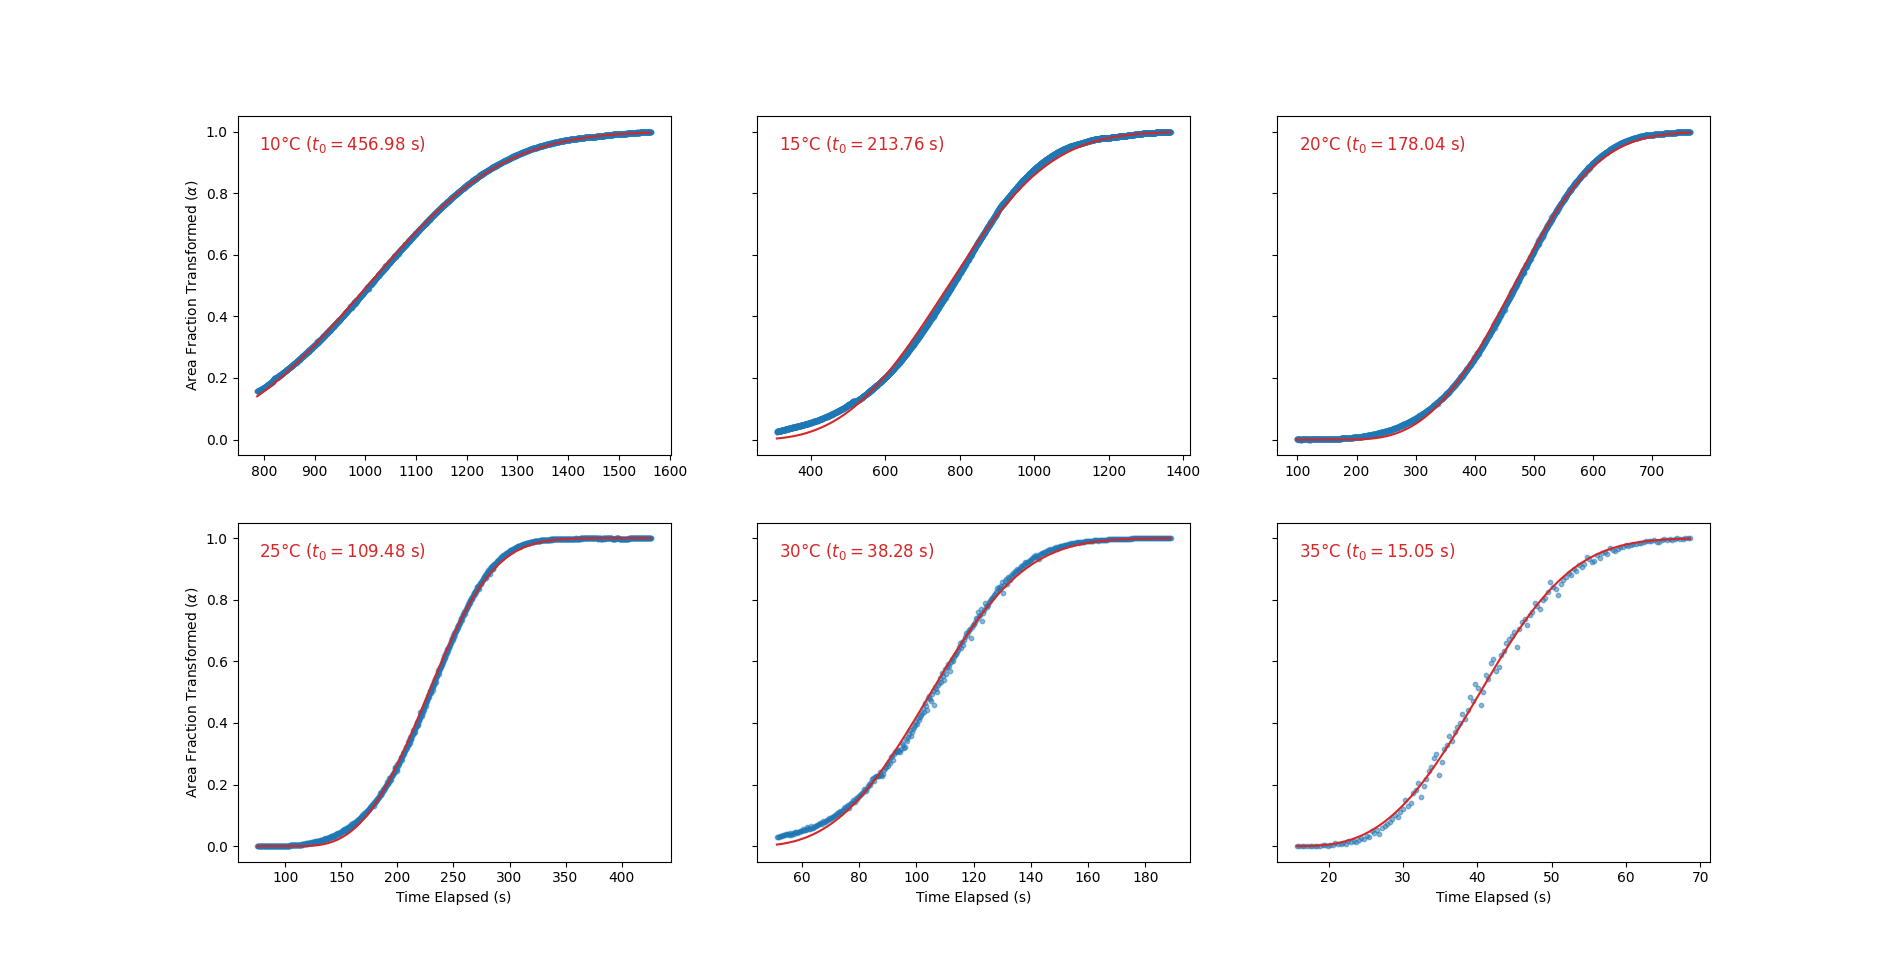
\includegraphics[width=1.0\linewidth]{jmak_1.png}
		\caption{}
		\label{fig:jmak_1}
	\end{figure}

NEED appendix figure containing the same information, but with all data points (highlighting those that were used for the fit) and the zero-value assigned point

\subsection{Microstructural Image Processing to Determine $\dot{N}/v$}

following the procedures of (cite papers here), a rudimentary algorithm was developed (largely ythrough trial and error) in order to process the microstructural images and count grains in a relaible manner...only the 140-micron images processed...the algorithm does the following using the skimage package:

1. merge the bright and dark field images, since it was observed that the bright field and dark field images highlighted different boundaries (boundary not visible in one might be visible in the other); dark field was simply converted to greyscale, while the bright field was converted to greyscale and the sobel gradient algorithm applied to locate boundaries...to "normalize" and to maximize contrast, the two images were then independently adjusted so that the middle 95\% of pixel intensities were stretched across the range [0, 1]...the maps were then averaged and the result inverted to create a map of grains, where dark regions are boundaries

2. so as to remove some noise and sharpen grain boundaries, gaussian smoothing was applied over cross-shaped pixel elements, followed by gaussian sharpening over a disk of radius 5 pixels

3. multiple otsu thresholding was used to sort the pixels into four different intensity bins; this was done so that small-angle grain boundaries (which were not as dark in the image) were caught by one of the intermediate bins, and the assumed grains corresponded only to the highest bin.

4. a "weighted opening" was executed, wherein the grains were eroded by a specified input radius, then dilated by half of that radius...the intermediate results were stacked, thereby creating a heatmap of the number of cycles required to eliminate any given pixel...essentially a smoothed version of calculating the distance to the nearest grain boundary

5. local maxima (of a radius specified by the minimum grain size) were counted as the locations of grains

6. for illustrative/diagnostic purposes, the watershed algorithm was used with the local maxima as markers and the heatmap as elevations in order to produce a grain map and assess the quality of the algorithm

input parameter (min grain size) as well as number of grains, grain densities are presented in TABLE ???, along with NV results of inputing into the result from JMAK theory

figure illustrating the process (bright field, dark field, merged map, multiple otsu, heatmap, grain map) for one of the samples, with all such diagrams contained in Appendix B

	\begin{figure}[h]
		\centering
		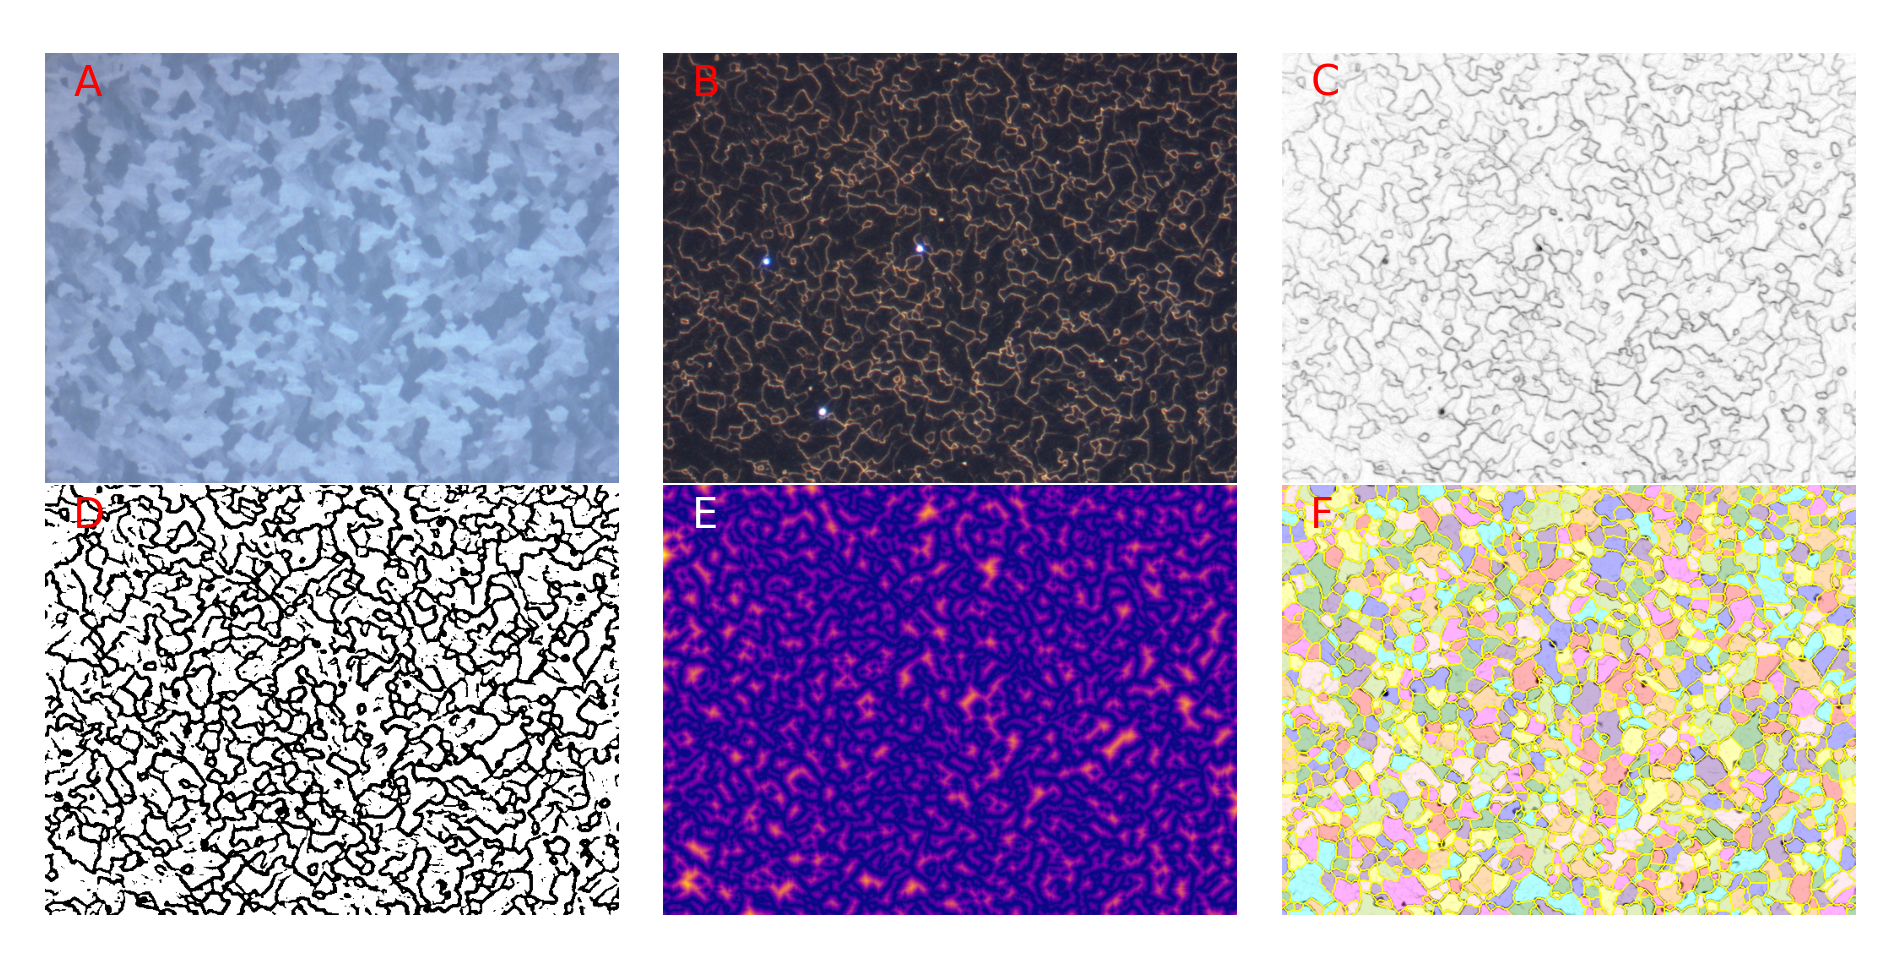
\includegraphics[width=1.0\linewidth]{microstructure_20C.png}
		\caption{}
		\label{fig:jmak_1}
	\end{figure}

discussion of the quality of the algorithm deferred for the Discussion, particularly with respect to the decision not to quantify error

\subsection{Calculation of Crystallization Parameters}

From Nv2 and N/v, N and v were obtained for each temperature. (Results summarized in TABLE ??)
  These values were then fit in 1/T-ln coordinates so as to estimate the prefactor and the activation energies; the results of which are contained in Figures ?? and ??.  All standard errorswere propagated according to equation ??.

TABLE containing results for T, N, v, standard errors

TABLE summarizing results of the fit (v0, N0, deltaG+Eattach, Eattach) and their uncertainties

FIGURE showing the fit results both in realspace and logspace

	\begin{figure}[h]
		\centering
		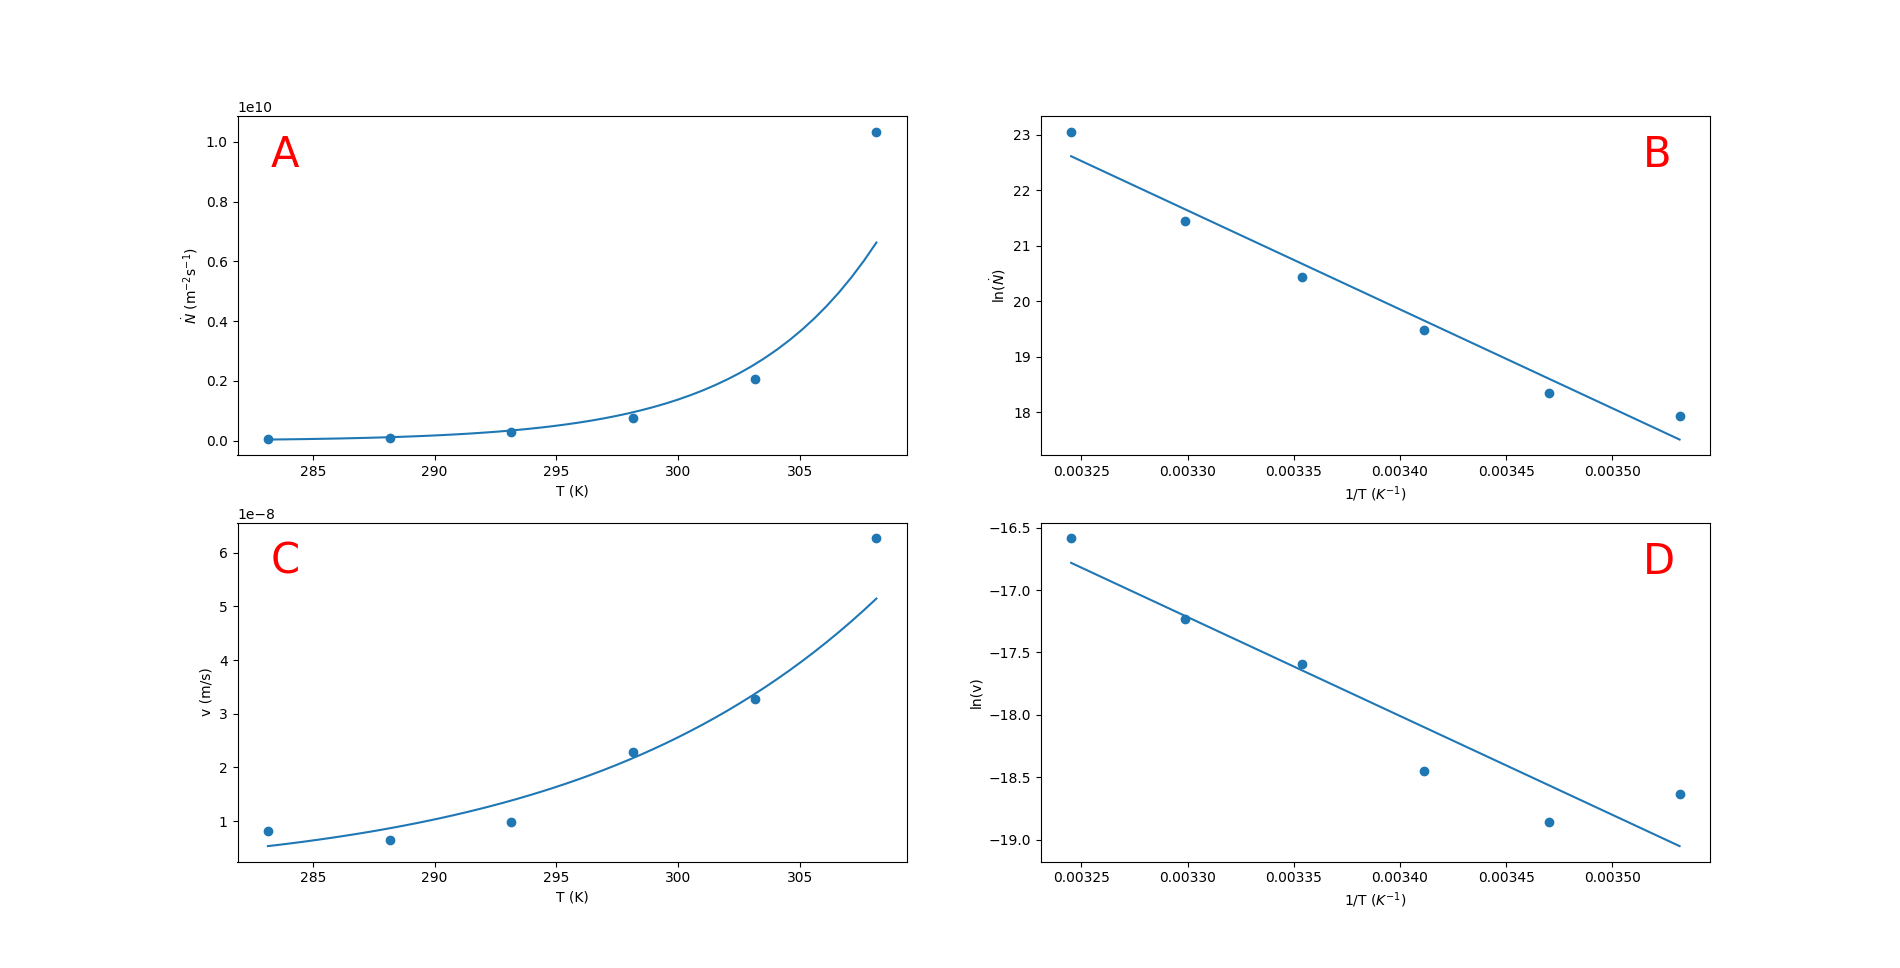
\includegraphics[width=1.0\linewidth]{linear_fits.png}
		\caption{}
		\label{fig:linear_fits}
	\end{figure}

subtracting the activation energies yields deltaG along with its standard error...of particular interest is the estimation of the critical cluster size and the free energy of crystallization g(c->a); however, as evidenced by the deltaG equation, this requires knowledge of the gamma factor.  A loose estimate may be obtained by the Materials Project in terms of average surface free energy; one would expect the corresponding free energy to be somewhere between this and zero...A spherical cluster is assumed, for which the nucleation barrier is typically calculated through EQUATION...recognizing that V=omega*ic, the critical radius is (), the critical area is (), we can rewrite this in the form EQUATION...gamma can therefore be calculated as EQUATION and, from the formula for critical nuclation energy of a spherical nucleus, g(c->a) can be calculated as ??...ic then can be calculated as EQUATION.  A plot of the relationship between the (unknown) surface energy of the crystalline-amorphous interface and the resulting critical nucleus size is shown in figure ???

FIGURE showing relationship between gamma and ic (atoms)

	\begin{figure}[h]
		\centering
		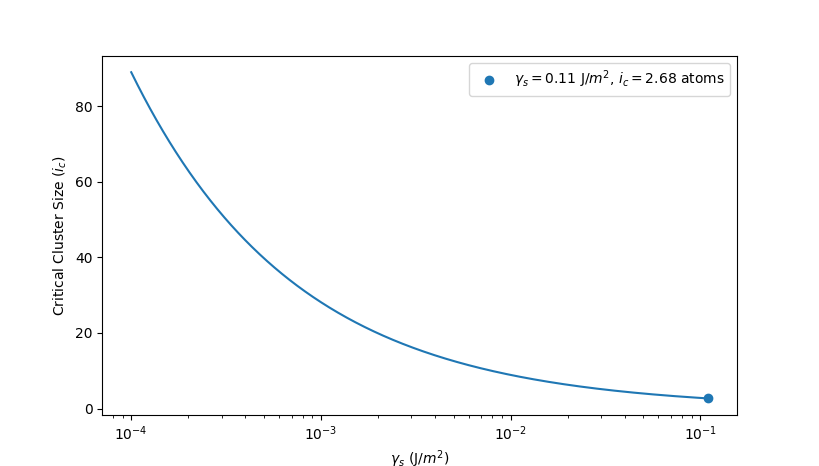
\includegraphics[width=1.0\linewidth]{cluster_size.png}
		\caption{}
		\label{fig:cluster_size}
	\end{figure}
